\documentclass[12pt, times new roman, a4paper]{article}
\usepackage[utf8]{inputenc}
\usepackage{graphicx}
\renewcommand{\figurename}{Gambar}

\title{Laporan Pemrograman}
\author{Ariq Rafi Kusumah}
\date{October 2019}

\begin{document}

\maketitle

\section{Teori}
\subsection{Sejarah Python}
	Python kembangkan oleh Guido van Rossum pada tahun 1990 di CWI. Am
sterdam kelanjutan dari bahasa pemrograman ABC.Versi yang terakhir dari
CWI 1.2 tahun 1995, Guido pindah ke CNRI versi yang dikeluarkan 1.6 tahun 2000. Guido dan pengembang inti pindah ke BeOpen.com perusahaan
komersial dan membentuk BeOpen PythonLabs dengan versi 2.0. Guido Pindah ke DigitalCreations. sekumpulan pemrograman yang dikoordinir Guido dan Python Software Foundation. Software Foundation adalah sebuah organisasinon-profit dengan versi 2.1 dan mencegah Python dimiliki oleh perusahaan komersial. Saat ini Pyhton sudah mencapai versi 2.7.13 dan versi 3.6.0.
\subsection{Perbedaan Python 2 dan 3}
\subsubsection{Syntax untuk mencetak teks}
Di Pyhton 2 perintah print menggunakan tandakurung dan tidak menggu
nakan kurung juga bisa di jalankan, contoh:\\
\\
print”Tidak Memakai kurung”\\
print(”Memakai Kurung”)\\
print”ini,;print”satu baris”\\
\\
Di Python 3 perintah print harus menggunakan tanda kurung, contoh:\\
\\
print(”Menggunakan Kurung”)\\
print(”digunakan untuk”,end=”)\\
print(”satu baris”)\\
\\
\subsubsection{Syntax Input}
Di Python 2 pada pemberian syntax input menggunakan raw dan menggu
nakan kutip satu,setelah itu print tidak memakai kurung contoh:\\
\\
nama=raw input(’Nama Anda:’)\\
print nama\\
\\
di Python 3 pada pemberian syntax iput menggunakan kutip dua dan tidak
menggunakan raw. setelah itu print menggunakan tanda kurung, contoh:\\
\\
nama=input(”Nama Anda:”)\\
print(nama)\\
\\
\subsubsection{Hasil Pembagian}
Di Python 2 setelah print tidak menggunakan tanda kurung. contoh:\\
\\
print ”3 / 2 = ” , 3/2\\
print ”3 // 2 = ” , 3//2\\
\\
Di Python 3 setelah print menggunakan tanda kurung. contoh :\\
\\
print (”3 / 2 = ” , 3/2)\\
print (”3 // 2 = ” , 3//2)\\
\\
\subsection{Python di Perusahaan Dunia}
\subsubsection{Google}
Dari awal berdiri, Google sudah menggunakan Python, bahkan Python merupakan salah satu bahasa pemrograman yang penting bagi Google, itulah mengapa Google pernah merekrut kreator Python Guido Van Rossum untuk bekerja di Google.\\

\noindent Sebuah kutipan dari pendiri Google “Python where we can, C++ where we must,” kutipan ini artinya jika menginginkan kontrol akan memori dan latensi yang rendah maka gunakan C++, sisanya gunakan Python sebisa mungkin, meskipun ada script yang ditulis untuk Google dalam bahasa Perl atau Bash, nantinya script tersebut akan diubah lagi ke Python, alasannya adalah karena kemudahan dalam perawatan.\\

\noindent Saat ini Python merupakan salah satu bahasa pemrograman server-side resmi di Google, selain Pyhton Google juga menggunakan C++, Java dan Go.
\subsubsection{Spotify}
Penyedia layanan musik streaming Spotify memanfaatkan Python untuk analisis data dan backend. Pada backend Spotify banyak terdapat service yang berkomunikasi lewat 0MQ (ZeroMQ) yang merupakan framework dan library open source untuk networking. 0MQ dibuat menggunakan Python dan C++. Alasan service dibuat menggunakan Python dikarenakan Spotify sangat menyukai kecepatan pipeline development.\\

\noindent Sistem rekomendasi Spotify bergantung pada analisis data yang sangat besar, untuk menginterpretasikan analisis tersebut Spotify menggunakan Luigi, modul Python yang sinkron dengan Hadoop. Modul open source ini menangani satu library dengan library lainnya agar saling bekerjasama, dan mengkonsolidasi eror log secara cepat.
\subsubsection{Instagram}
Seperti yang kita ketahui, Instagram telah merevolusi komunikasi visual dan pemasaran digital melalui media foto. Dengan 400 juta pengguna aktif setiap harinya, tentu ini menghapus pendapat yang mengatakan bahwa aplikasi python tidak terlalu scalable. Menurut Hui Ding, engineer di Instagram, moto para pengembang aplikasi di instagram adalah “Do the simple thing first,” dan hal ini sangat bisa dilakukan menggunakan Python, bagi para pengembang aplikasi di Instagram Python sangat ramah pengguna, sederhana dan rapi. Juga karena Python sangat populer, maka tidaklah sulit menemukan pengembang baru untuk memperbesar tim.
\subsubsection{Industrial Light and Magic}
ILM adalah Studio spesial-efek yang didirikan oleh George Lucas pada tahun 1975, awalnya studio ini membuat berbagai efek yang dibutuhkan untuk film Star Wars saja, namun studio ini berkembang pesat dan meraih banyak penghargaan. Seiring berkembangnya teknologi komputer , ILM meyakini bahwa CGI merupakan masa depan bagi efek visual dan mulai mencari sistem yang tepat. Karena infrastruktur awal ILM dibuat menggunakan C dan C++, maka akan lebih mudah mengintegrasikan Python ketimbang Perl ataupun Tcl. Menggunakan Python, ILM dapat dengan mudah membungkus komponen software dan meningkatkan aplikasi grafis mereka. Hingga saat ini ILM tetap menggunakan Python karena selalu dapat menghadirkan solusi terbaik untuk kebutuhan mereka.
\subsubsection{Netflix}
Salah satu penggunaan utama Python di aplikasi Netflix adalah pada Central Alert Gateway. Aplikasi RESTful ini akan me-reroute alert dan mengirimkannya pada kelompok atau individu yang berhak melihatnya. Sebagai tambahan aplikasi ini akan secara otomatis reboot atau menghentikan proses yang dianggap bermasalah. Selain C.A.G, Python juga digunakan pada aplikasi untuk menelusuri riwayat dan perubahan pengaturan keamanan.
\\
\\
\\
\\
\\
\\
\\
\\
\\
\\
\\
\\
\\
\section{Instalasi}
\subsection{Anaconda versi 3}
1. Klik Next\\ 
\begin{figure}[h]
	\centering
		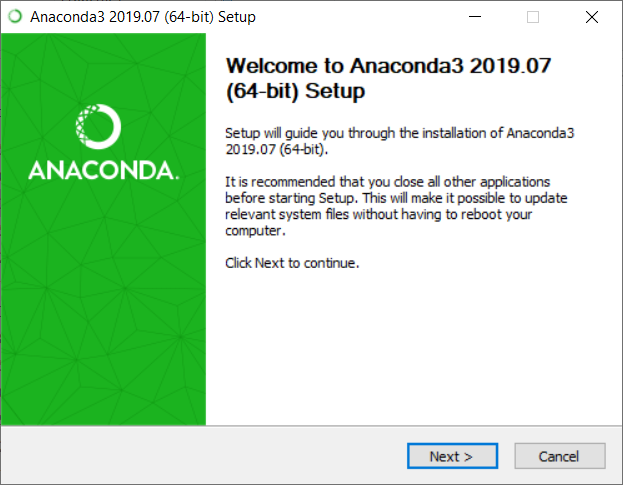
\includegraphics[scale=0.5]{Gambar/A1}
	\caption{Klik Next}
\end{figure}
\\
2. Klik I Agree\\
\begin{figure}[h]
	\centering
		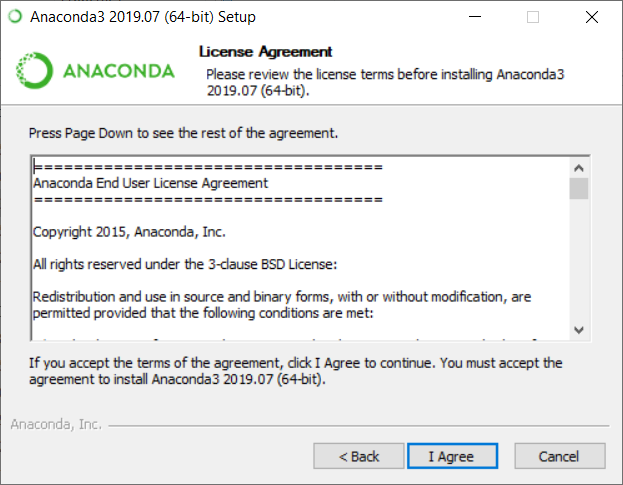
\includegraphics[scale=0.5]{Gambar/A2}
	\caption{Klik Agree}
\end{figure}
\\
\\
\\
\\
\\
\\
\\
3. Pilih Just me, Lalu Klik Next\\
\begin{figure}[h]
	\centering
		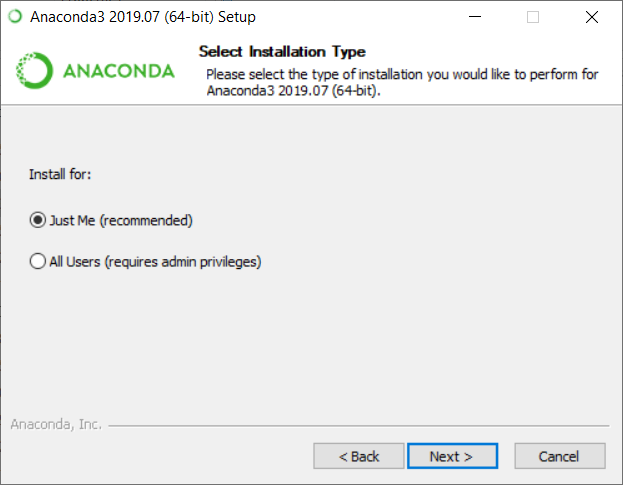
\includegraphics[scale=0.5]{Gambar/A3}
	\caption{Klik I Agree}
\end{figure}
\\
4. Pilih lokasi penyimpanan sesuai dengan keinginan kalian, lalu Klik Next\\
\begin{figure}[h]
	\centering
		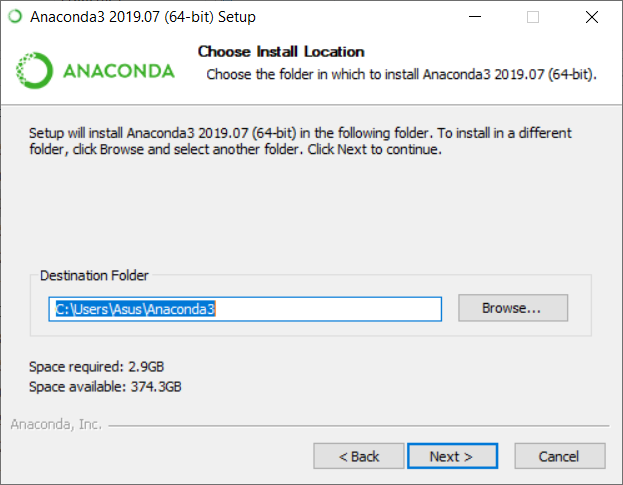
\includegraphics[scale=0.5]{Gambar/A4}
	\caption{Choose Install Location}
\end{figure}
\\
\\
\\
\\
\\
\\
\\
\\
\\
\\
5. Ceklis keduanya untuk melalukan PATH dan Register\\
\begin{figure}[h]
	\centering
		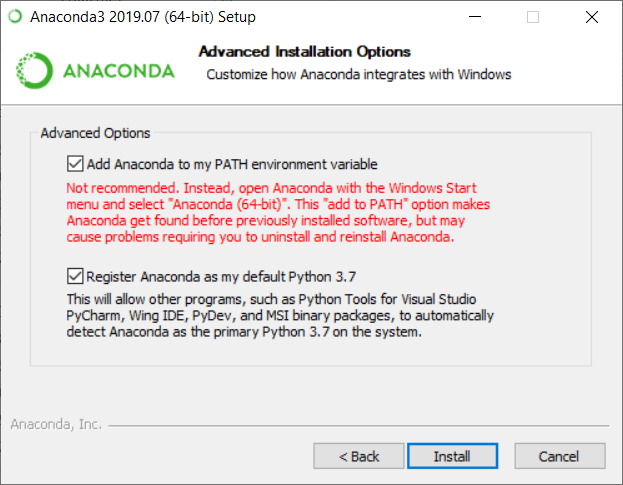
\includegraphics[scale=0.5]{Gambar/A5}
	\caption{Advanced Installation Options}
\end{figure}
\\
6. Tunggu Proses Instalan\\
\begin{figure}[h]
	\centering
		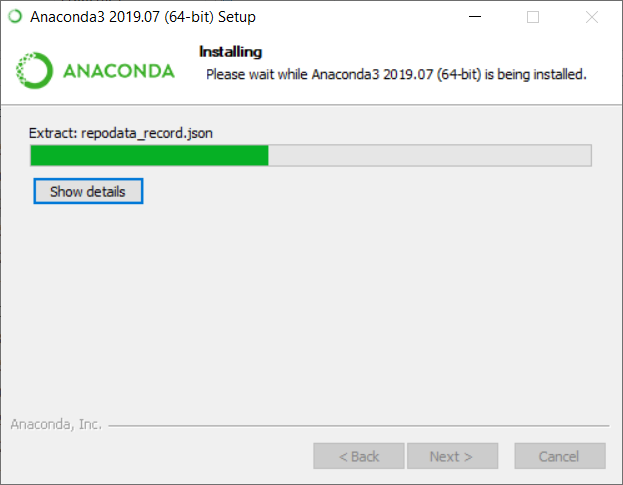
\includegraphics[scale=0.5]{Gambar/A6}
	\caption{Installing}
\end{figure}
\\
\\
\\
\\
\\
\\
\\
\\
\\
\\
7. Setelah Complate, Klik Next\\
\begin{figure}[h]
	\centering
		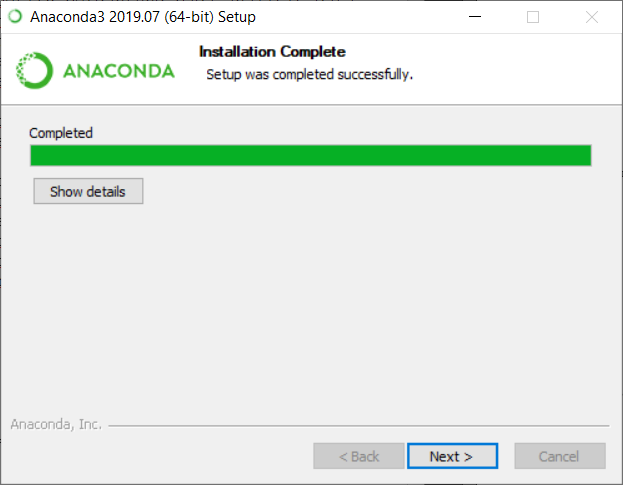
\includegraphics[scale=0.5]{Gambar/A7}
	\caption{Installation Complate}
\end{figure}
\\
8. Lalu Klik Next\\
\begin{figure}[h]
	\centering
		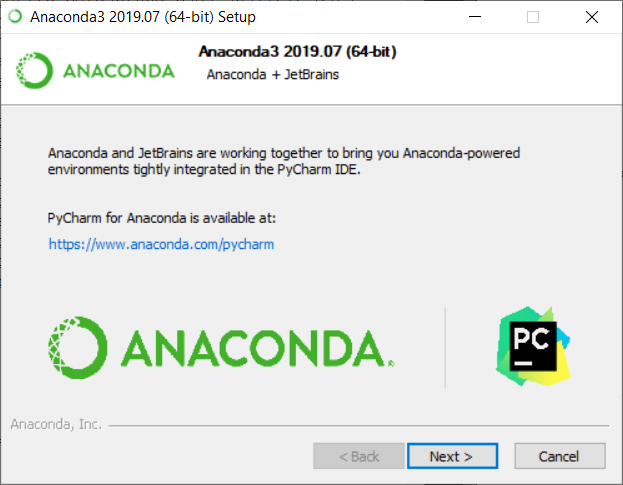
\includegraphics[scale=0.5]{Gambar/A8}
	\caption{Anaconda3 2019.07}
\end{figure}
\\
\\
\\
\\
\\
\\
\\
\\
\\
\\
9. Selesai\\
\begin{figure}[h]
	\centering
		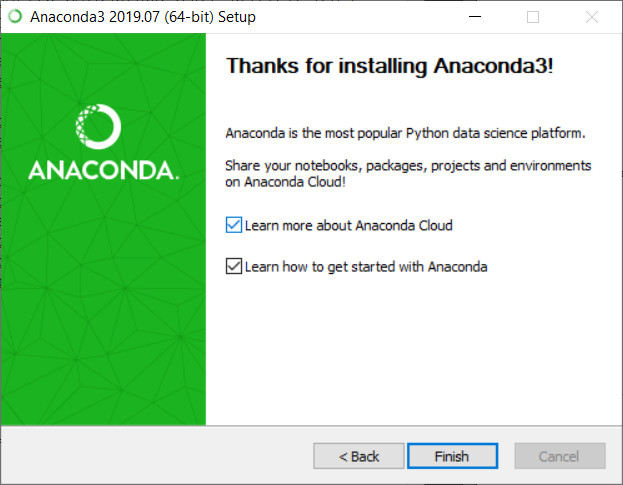
\includegraphics[scale=0.5]{Gambar/A9}
	\caption{Thanks for installing Anaconda 3}
\end{figure}
\\
\subsection{Install PIP}
1. Download di browser \textbf{get.pip}, lalu simpan di Desktop.\\
2. Buka CMD , Lalu ketikan di cmd pip -V untuk mengecek versi pip, setelah itu cd desktop, lalu ketikan python get-pip.py\\
\begin{figure}[h]
	\centering
		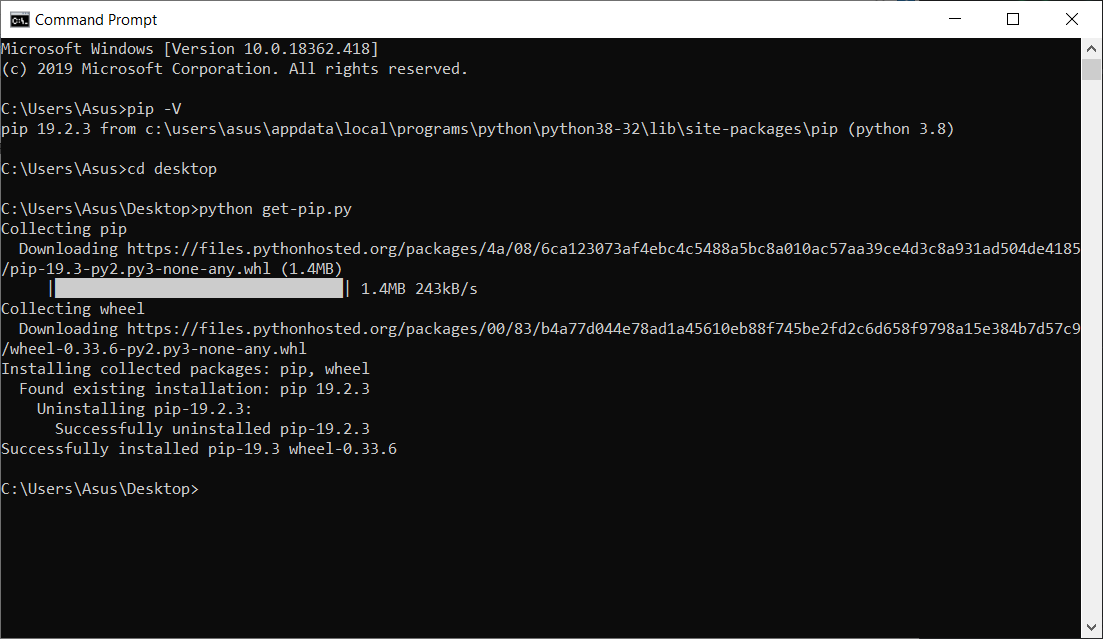
\includegraphics[scale=0.5]{Gambar/C1}
		\caption{PIP}
\end{figure}
\\
\section{Cara Setting Environment}

\section{Entrepreter/CLI}
1. Pertama buka CMD\\
2. ketikan python , ketikan seperti gambar di bawah :\\
\begin{figure}[h]
	\centering
		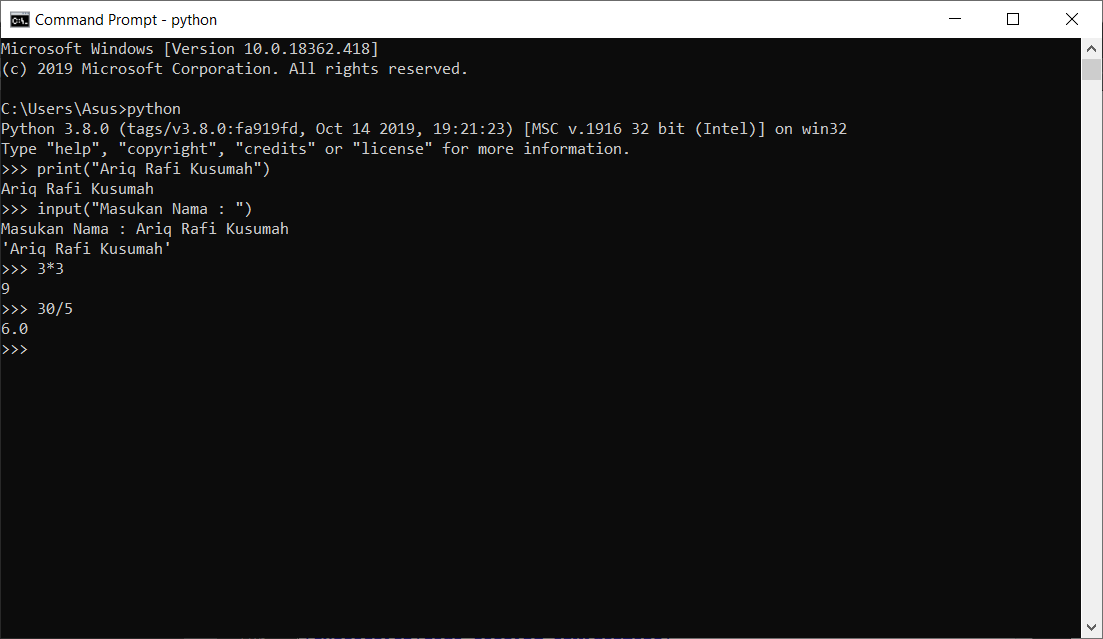
\includegraphics[scale=0.5]{Gambar/CLI}
	\caption{CLI}
\end{figure}
\\
\\
\\
\\
\\
\\
\\
\\
\\
\\
\\
\section{Menjalankan dan mengupdate anaconda dan spyder}
1. Buka CMD dan ketikan \textbf{conda install -c anaconda python}\\
\begin{figure}[h]
	\centering
		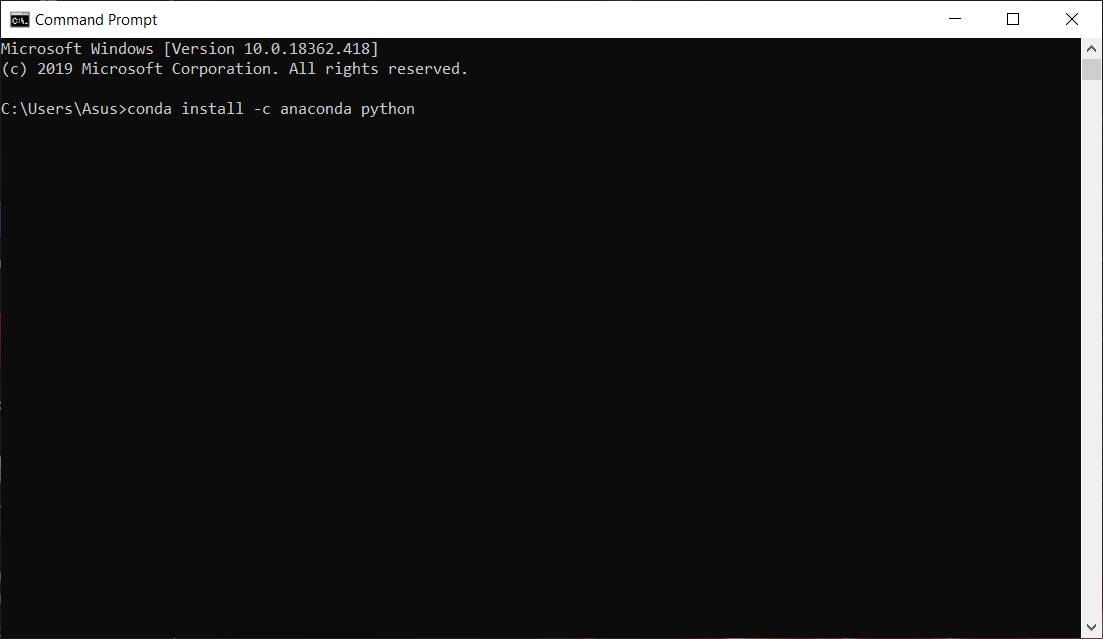
\includegraphics[scale=0.4]{Gambar/U1}
	\caption{Update 1}
\end{figure}
\\
2. Tekan Y/y untuk melanjutkan update\\
\begin{figure}[h]
	\centering
		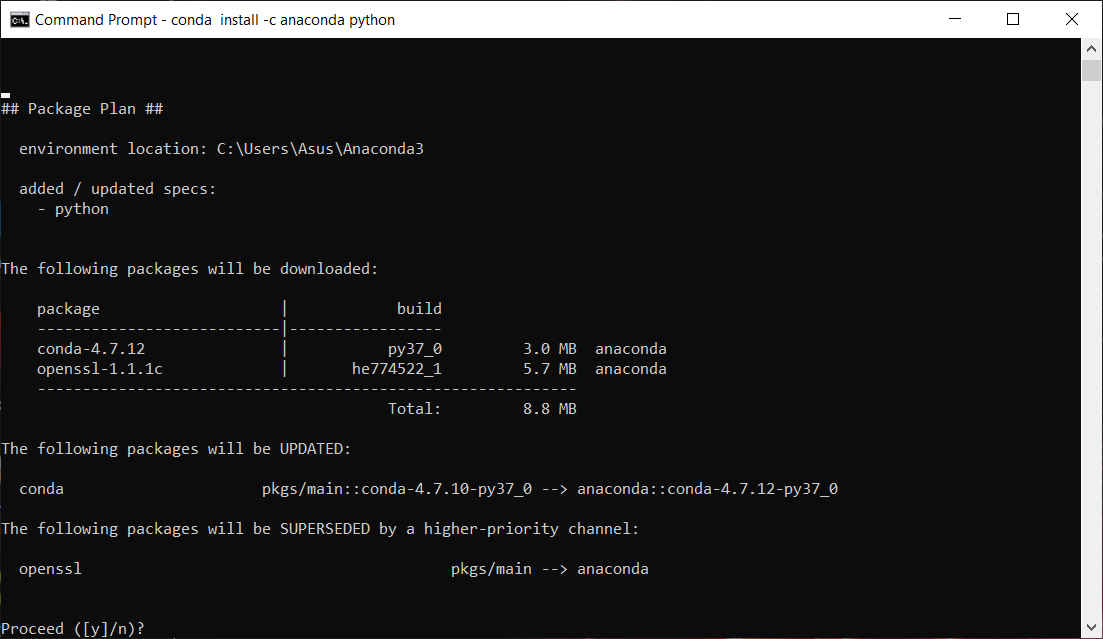
\includegraphics[scale=0.4]{Gambar/U2}
	\caption{Update 2}
\end{figure}
\\
3. Buka Spyder untuk mengecek versinya\\
\begin{figure}[h]
	\centering
		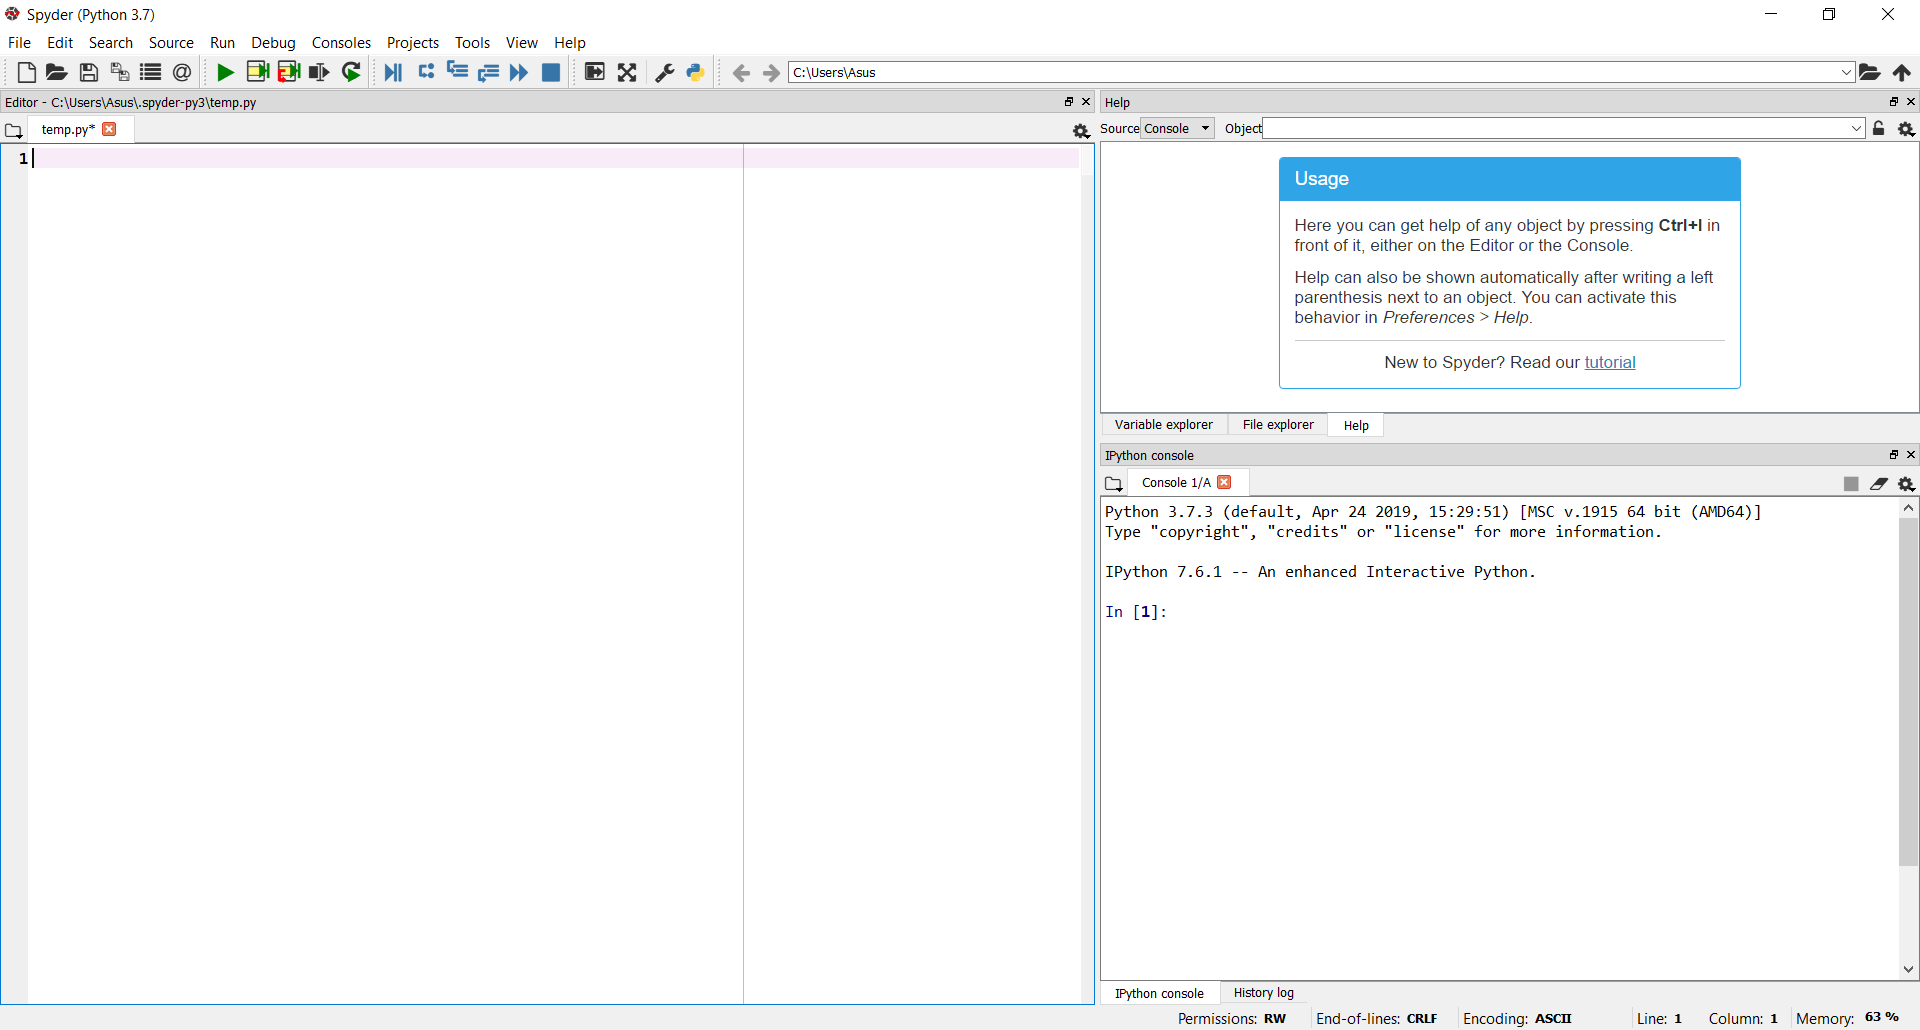
\includegraphics[scale=0.2]{Gambar/U3}
		\caption{Update 3}
\end{figure}
\section{Menjalankan Script Hello World di Spyder}
1. Buka Anaconda 3 , Lalu pilih Launch Sypder.\\
\begin{figure}[h]
	\centering
		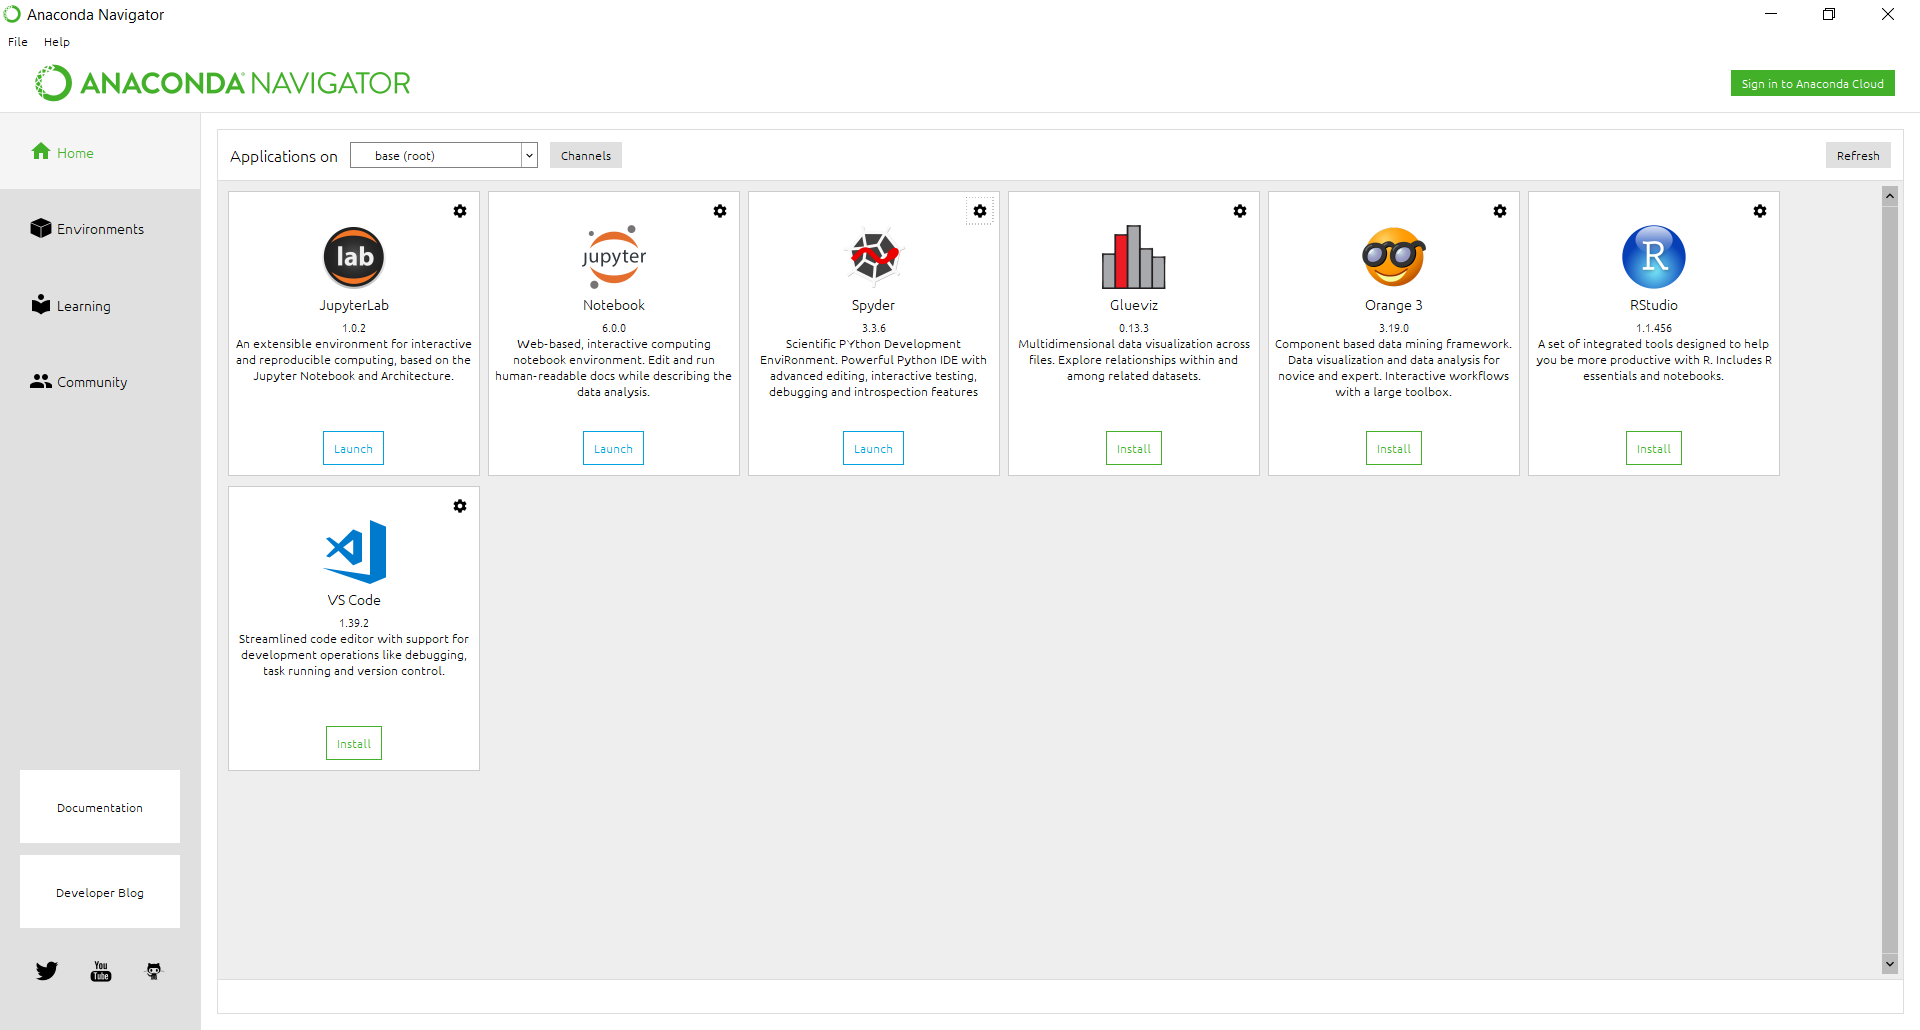
\includegraphics[scale=0.2]{Gambar/S1}
		\caption{Spyder}
\end{figure}
\\
2. Ketik seperti dibawah ini, lalu Klik Run.\\
\begin{figure}[h]
	\centering
		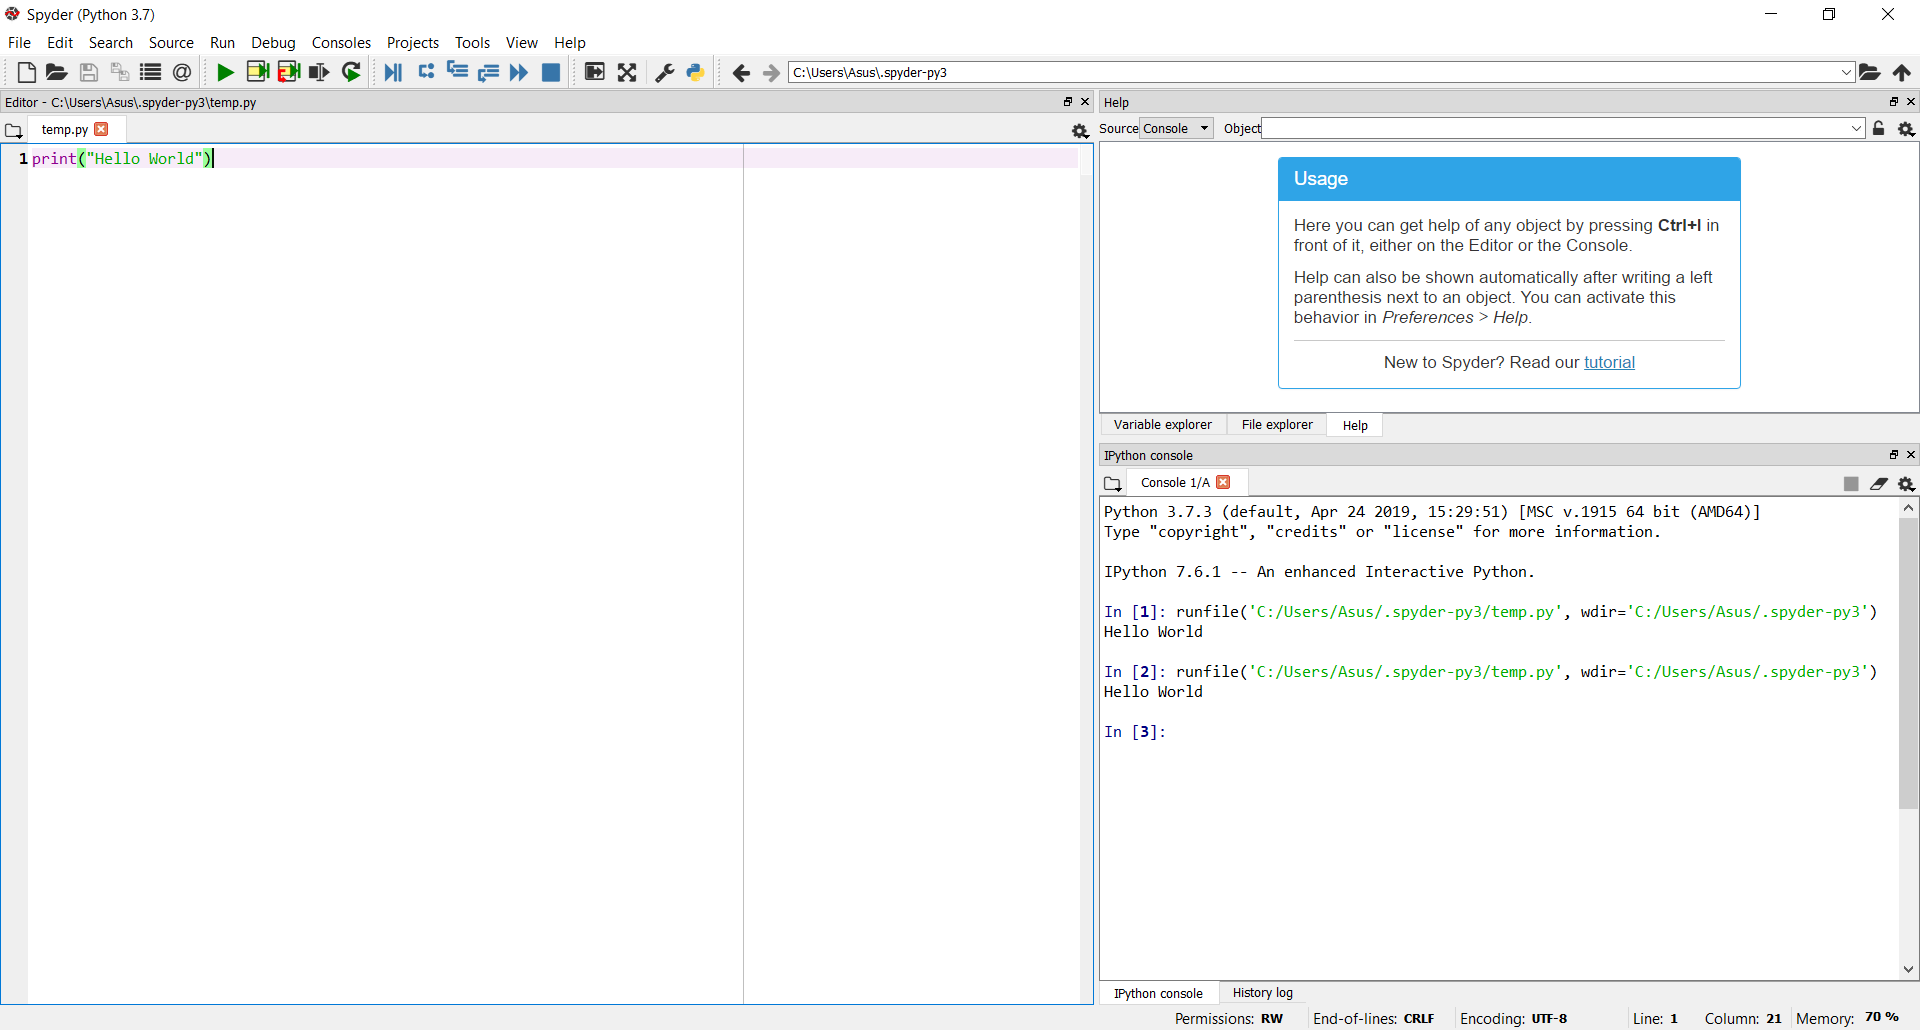
\includegraphics[scale=0.2]{Gambar/S2}
	\caption{Hellow World}
\end{figure}
\\
\\
\section{Cara menjalankan Script otomatis login aplikasi akademik dengan library selenium dan inputan user}

\section{Cara pemakaian variable explorer di spyder}
1. Buka Spyder\\
2. Ketikan Seperti di gambar ini\\
\begin{figure}[h]
	\centering
		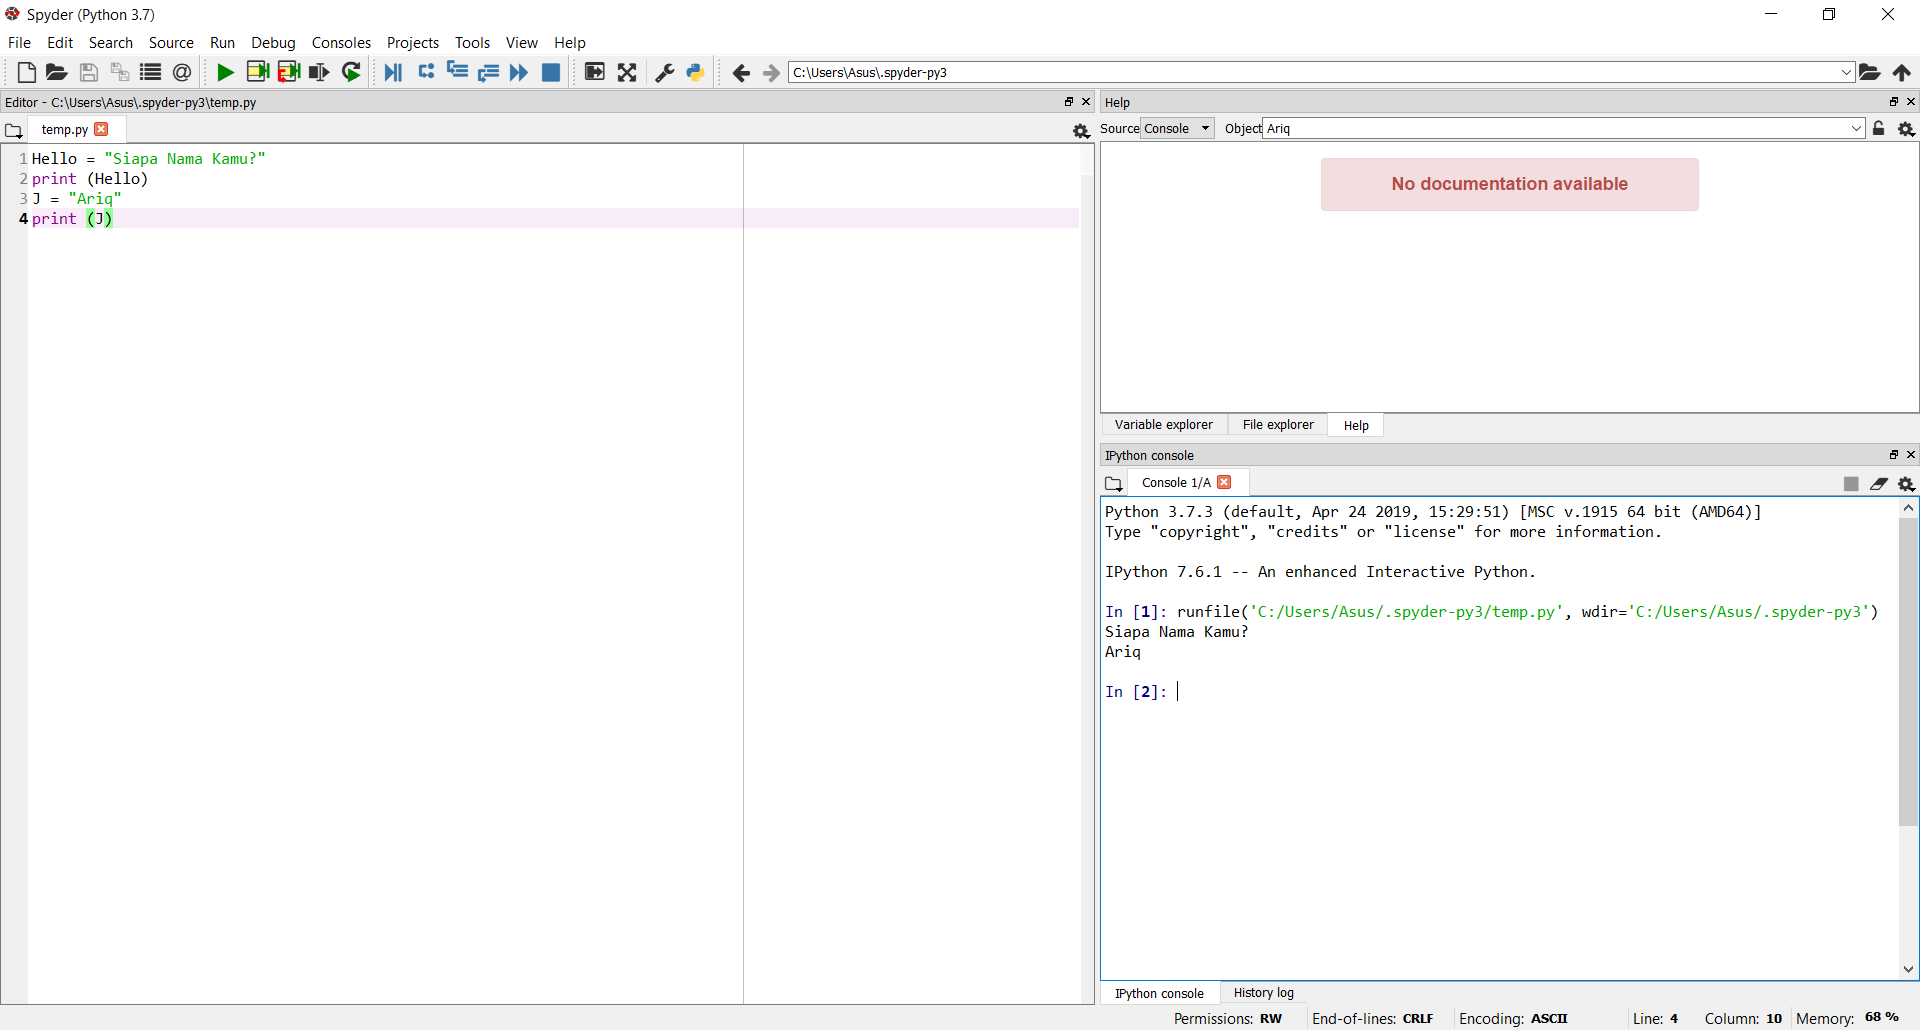
\includegraphics[scale=0.2]{Gambar/V1}
	\caption{Variable}
\end{figure}
\\
\section{Penjelasan Identasi}
Identasi adalah bagian dari suatu paragraf yang menjorok kedalam pada baris tiap paragraf. Mengatur indentasi dengan cara menggunakan tab atau spasi. Identasi digunakan oleh bahasa pemrograman python sebagai pengganti briket () untuk membuka dan menutup suatu fungsi. Error indentasi dapat terjadi jika syntax tidak menggunakan tab atau space.

\section{jenis jenis error identasi yang didapat}
1. Jenis codingan yang menjorok kedalam , dapat menyebabkan error.\\
\begin{figure}[h]
	\centering
		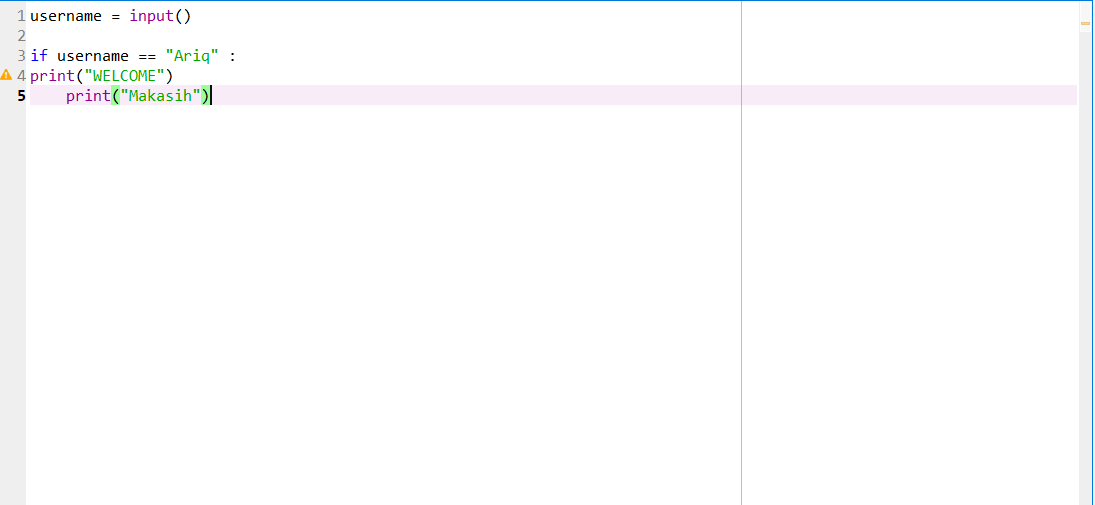
\includegraphics[scale=0.4]{Gambar/E1}
	\caption{Error1}
\end{figure}
\\
2. Run Program , maka hasilnya 	Error\\
\begin{figure}[h]
	\centering
		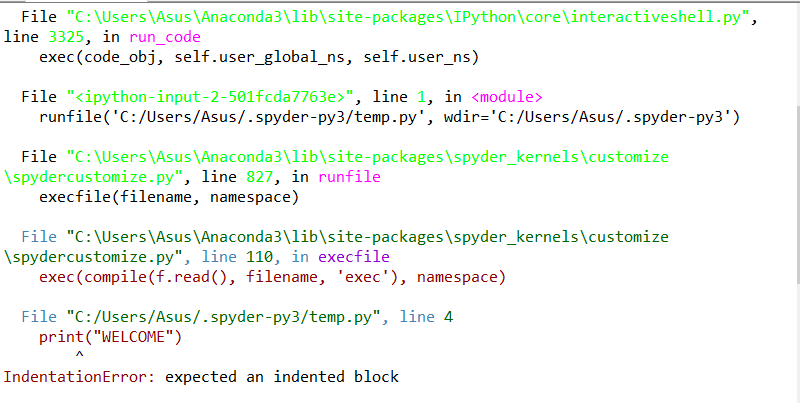
\includegraphics[scale=0.5]{Gambar/E2}
	\caption{Error2}
\end{figure}
\\
\section{cara membaca error}
1. Coding yang tidak bisa di run, dan ada tanda warning di samping.
\begin{figure}[h]
	\centering
		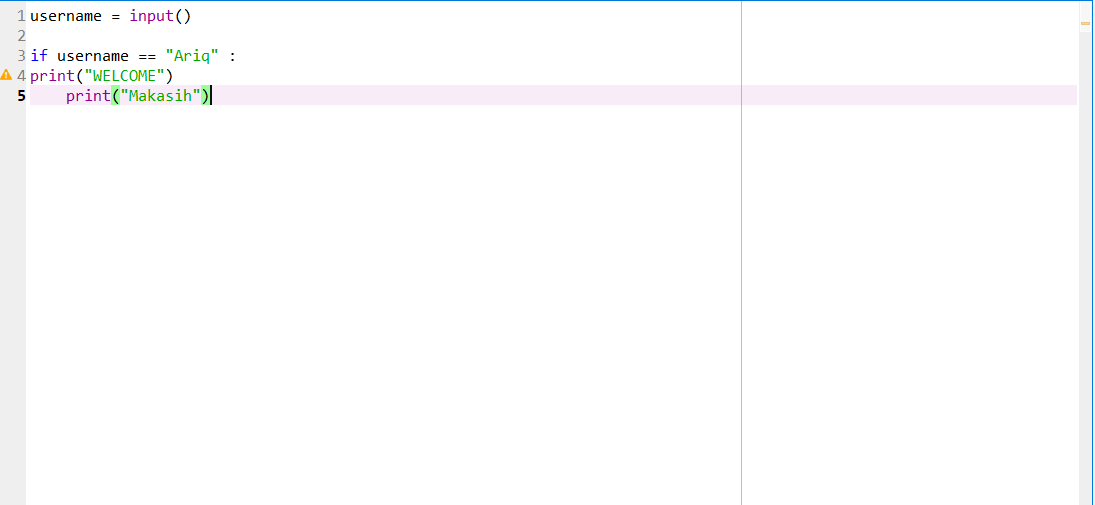
\includegraphics[scale=0.4]{Gambar/E1}
	\caption{Membaca error}
\end{figure}
\\
2. Maka akan tulisan seperti ini jika di run.\\
\begin{figure}[h]
	\centering
		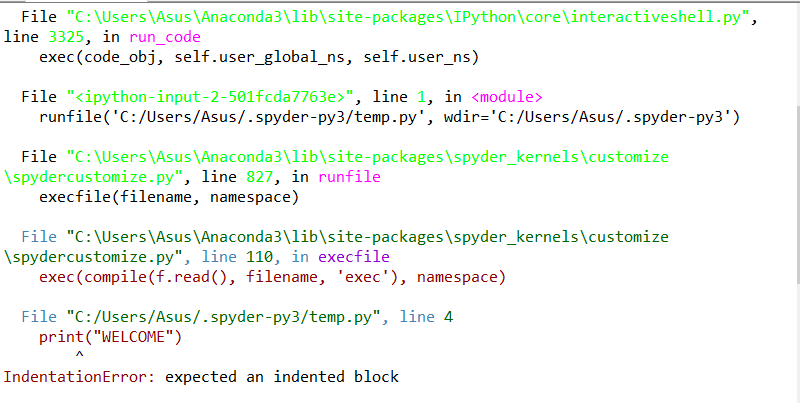
\includegraphics[scale=0.5]{Gambar/E2}
	\caption{Hasil Run}
\end{figure}
\\
\\
\\
\\
\\
\\
\\
\\
\\
\section{cara menangani errornya}
1. Lihat line berapa yang menandakan error , lalu tekan TAB atau spasi.
\begin{figure}[h]
	\centering
		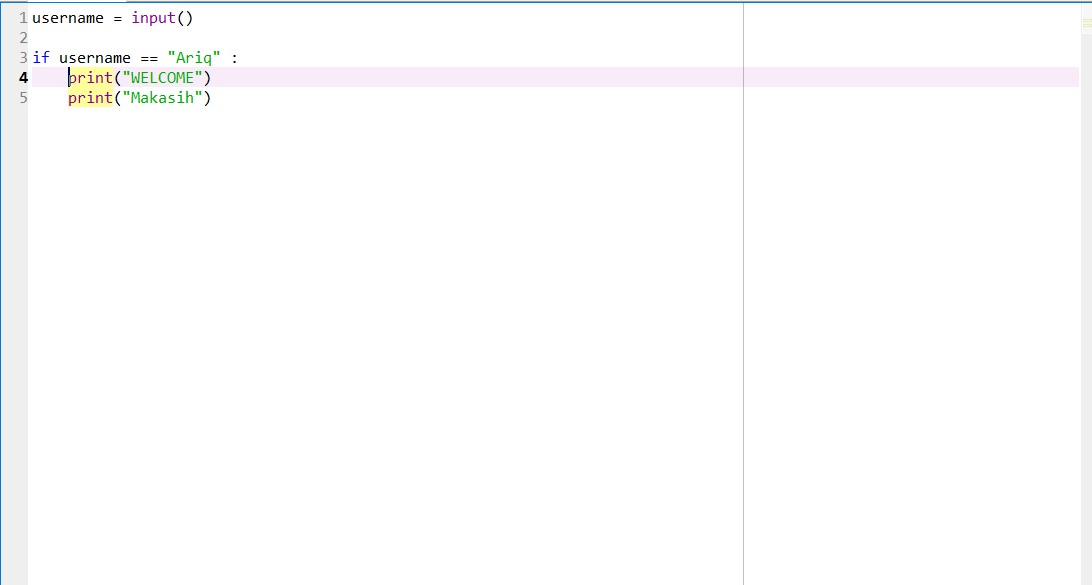
\includegraphics[scale=0.4]{Gambar/E3}
	\caption{Sudah Di Edit}
\end{figure}

\end{document}
